%thesis.tex 
%Model LaTeX file for Ph.D. thesis at the 
%School of Mathematics, University of Edinburgh


\documentclass[11pt,a4paper,openright]{article}

%\usepackage{url,graphicx}

\usepackage{amsmath}
%\usepackage{natbib}
\usepackage{booktabs}
\usepackage{graphicx}
\usepackage{hyperref}%backref,
%\usepackage[dvips]{color}
\graphicspath{{expt/}}


\usepackage{times}
\usepackage[varg]{txfonts}

%%% Macro definitions for Commonly used symbols
\newcommand{\etas}{\ensuremath{\eta_{\mathrm{s}}}}
%\documentclass[a4paper, 11pt, draft]{Thesis} 

\usepackage{etex}
\usepackage{fixltx2e}
\usepackage{color,soul}
% This file contains macros that can be called up from connected TeX files
% It helps to summarise repeated code, e.g. figure insertion (see below).

% insert a centered figure with caption and description
% parameters 1:filename, 2:title, 3:description and label
\newcommand{\figuremacro}[3]{
	\begin{figure}[H]
		\centering
		\includegraphics[width=1\textwidth]{#1}
		\caption[#2]{\textbf{#2} - #3}
		\label{#1}
	\end{figure}
}

% insert a centered figure with caption and description AND WIDTH
% parameters 1:filename, 2:title, 3:description and label, 4: textwidth
% textwidth 1 means as text, 0.5 means half the width of the text
\newcommand{\figuremacroW}[4]{
	\begin{figure}[H]
		\centering
		\includegraphics[width=#4\textwidth]{#1}
		\caption[#2]{\textbf{#2} - #3}
		\label{#1}
	\end{figure}
}

% insert a figure with sub figures caption and description
% parameters 1:filename_1, 3:title and descriptionl_1,
% 3:filename_2, 4:title and descriptionl_2,  
% 5:title_main, 6:description and label_main,
% Each subfigure has its own caption
\newcommand{\figuremacroSubTwo}[6]{
	\begin{figure}[H]
	        \centering
		\begin{minipage}[b]{0.475\textwidth}
			\centering
			\includegraphics[width=\textwidth]{#1}
			\subcaption{#2}
		\end{minipage}%
		~
		\begin{minipage}[b]{0.475\textwidth}
			\centering
			\includegraphics[width=\textwidth]{#3}
			\subcaption{#4}
		\end{minipage}%
		\caption[#5]{\textbf{#5} - #6}
		\label{#5}
	\end{figure}
}

% insert a figure with sub figures caption and description
% parameters 1:filename_1, 3:title and descriptionl_1,
% 3:filename_2, 4:title and descriptionl_2,  
% 5:title_main, 6:description and label_main,
% Each subfigure has its own caption
\newcommand{\figuremacroSubTwoBS}[6]{
	\begin{figure}[H]
	        \centering
		\begin{minipage}[b]{0.3\textwidth}
			\centering
			\includegraphics[width=\textwidth]{#1}
			\subcaption{#2}
		\end{minipage}%
		~
		\begin{minipage}[b]{0.65\textwidth}
			\centering
			\includegraphics[width=\textwidth]{#3}
			\subcaption{#4}
		\end{minipage}%
		\caption[#5]{\textbf{#5} - #6}
		\label{#5}
	\end{figure}
}

% insert a figure with sub figures caption and description
% parameters 1:filename_1, 3:title and descriptionl_1,
% 3:filename_2, 4:title and descriptionl_2,  
% 5:title_main, 6:description and label_main,
% Each subfigure has its own caption
\newcommand{\figuremacroSubThree}[8]{
	\begin{figure}[H]
	        \centering
		\begin{minipage}[b]{0.3\textwidth}
			\centering
			\includegraphics[width=\textwidth]{#1}
			\subcaption{#2}
		\end{minipage}%
		~
		\begin{minipage}[b]{0.3\textwidth}
			\centering
			\includegraphics[width=\textwidth]{#3}
			\subcaption{#4}
		\end{minipage}%
		~
		\begin{minipage}[b]{0.3\textwidth}
					\centering
					\includegraphics[width=\textwidth]{#5}
					\subcaption{#6}
		\end{minipage}%
		\caption[#7]{\textbf{#7} - #8}
		\label{#7}
	\end{figure}
}

% insert a figure with sub figures caption and description
% parameters 1:filename_1, 3:title and descriptionl_1,
% 3:filename_2, 4:title and descriptionl_2,  
% 5:title_main, 6:description and label_main,
% Each subfigure has its own caption
\newcommand{\figuremacroSubFour}[9]{
	\begin{figure}[H]
	        \centering
	
		\begin{minipage}[b]{0.235\textwidth}
			\centering
			\includegraphics[width=\textwidth]{#1}
			\subcaption{#2}
		\end{minipage}%
		~
		\begin{minipage}[b]{0.235\textwidth}
			\centering
			\includegraphics[width=\textwidth]{#3}
			\subcaption{#4}
		\end{minipage}%
		~
		\begin{minipage}[b]{0.235\textwidth}
			\centering
			\includegraphics[width=\textwidth]{#5}
			\subcaption{#6}
		\end{minipage}%
		~
		\begin{minipage}[b]{0.235\textwidth}
			\centering
			\includegraphics[width=\textwidth]{#7}
			\subcaption{#8}
		\end{minipage}%				
		\caption[#9]{\textbf{#9}}
		\label{#9}
	\end{figure}
}


% insert 2 figures caption and description side by side
% parameters 1:filename_1, 2:title_1, 3:description and label_1, 
% 1:filename_2, 2:title_2, 3:description and label_2,
% Each subfigure has
\newcommand{\figuremacroSBSTwo}[6]{
	\begin{figure}[H]
	        \centering
			\begin{minipage}{.44\textwidth}
			\centering
			\includegraphics[width=\textwidth]{#1}
			\caption[#2]{\textbf{#2} - #3}
			\label{#1}
		\end{minipage}%
		~
		\begin{minipage}{.44\textwidth}
			\centering
			\includegraphics[width=\textwidth]{#4}
			\caption[#5]{\textbf{#5} - #6}
			\label{#4}
		\end{minipage}%
	\end{figure}
}


% insert 2 figures caption and description side by side
% parameters 1:filename_1, 2:title_1, 3:description and label_1, 
% 1:filename_2, 2:title_2, 3:description and label_2,
% Each subfigure has
\newcommand{\figuremacroSBSThree}[9]{
	\begin{figure}[H]
	        \centering
			\begin{minipage}{.31\textwidth}
			\centering
			\includegraphics[width=\textwidth]{#1}
			\caption[#2]{\textbf{#2} - #3}
			\label{#1}
		\end{minipage}%
		~
		\begin{minipage}{.31\textwidth}
			\centering
			\includegraphics[width=\textwidth]{#4}
			\caption[#5]{\textbf{#5} - #6}
			\label{#4}
		\end{minipage}%
			~
		\begin{minipage}{.31\textwidth}
					\centering
					\includegraphics[width=\textwidth]{#7}
					\caption[#5]{\textbf{#8} - #9}
					\label{#7}
		\end{minipage}%
	\end{figure}
}

% inserts a figure with wrapped around text; only suitable for NARROW figs
% o is for outside on a double paged document; others: l, r, i(inside)
% text and figure will each be half of the document width
% note: long captions often crash with adjacent content; take care
% in general: above 2 macro produce more reliable layout
\newcommand{\figuremacroN}[3]{
	\begin{wrapfigure}{o}{0.5\textwidth}
		\centering
		\includegraphics[width=0.48\textwidth]{#1}
		\caption[#2]{{\small\textbf{#2} - #3}}
		\label{#1}
	\end{wrapfigure}
}



% predefined commands by Harish
\newcommand{\PdfPsText}[2]{
  \ifpdf
     #1
  \else
     #2
  \fi
}

\newcommand{\IncludeGraphicsH}[3]{
  \PdfPsText{\includegraphics[height=#2]{#1}}{\includegraphics[bb = #3, height=#2]{#1}}
}

\newcommand{\IncludeGraphicsW}[3]{
  \PdfPsText{\includegraphics[width=#2]{#1}}{\includegraphics[bb = #3, width=#2]{#1}}
}

\newcommand{\InsertFig}[3]{
  \begin{figure}[!htbp]
    \begin{center}
      \leavevmode
      #1
      \caption{#2}
      \label{#3}
    \end{center}
  \end{figure}
}


%%% Local Variables: 
%%% mode: latex
%%% End: 
 % This file adds the macros for adding figures
  
% Include any extra LaTeX packages required
\usepackage[square, authoryear, colon, sort&compress]{natbib}  % Use the "Natbib" style for the references in the Bibliography
%\usepackage{verbatim}  % Needed for the "comment" environment to make LaTeX comments
\usepackage{vector}  % Allows "\bvec{}" and "\buvec{}" for "blackboard" style bold vectors in maths
\usepackage{float}
\usepackage{ifpdf}

%%% Some Fonts
\usepackage{textcomp}
\usepackage{pifont}% http://ctan.org/pkg/pifont
\usepackage{needspace}
\usepackage[noabbrev]{cleveref} %For crossreferencing

\usepackage{etoolbox}
\usepackage{float}

%%% For Changing fonts
%\usepackage[utf8]{inputenc}
\usepackage[T1]{fontenc}
\usepackage{charter}
%\usepackage[expert]{mathdesign}

%%% Packages for tables
\usepackage[usenames,dvipsnames,table]{xcolor}
\usepackage{hyperref}
\definecolor{red}{RGB}{255,50,50}
\definecolor{light_orange}{RGB}{253,245,230}
\definecolor{gray}{RGB}{225,225,225}
\usepackage{colortbl}% Allows shading of table cells
% Define a simple command to use at the start of a table row to make it have a shaded background
%\newcommand{\gray}{\rowcolor[gray]{.9}}

% % % Packages for TikZ setup for diagrams
%\usepackage[mode=buildnew]{standalone}
%%\standaloneconfig{mode=buildnew}
%\usepackage{tikz,pgfplots}
%\pgfplotsset{compat=newest}
%\usetikzlibrary{shapes,shapes.multipart,shapes.misc,shapes.geometric,arrows,shapes.symbols,shadows,shadows.blur}
%\usepackage{arydshln}
\usepackage{bm}
%\usepackage{tocbibind} 
%\renewcommand{\refname}{References}
%\renewcommand{\bibname}{References}

%:-------------------------- packages for fancy things -----------------------

%%% A (page...) to backref
\makeatletter
\patchcmd{\BR@backref}{\newblock}{\newblock(p.~}{}{}
\patchcmd{\BR@backref}{\par}{)\par}{}{}
\makeatother

%Make equation number label bold
\makeatletter
\let\mytagform@=\tagform@
\def\tagform@#1{\maketag@@@{\bfseries(\ignorespaces#1\unskip\@@italiccorr)}\hspace{3mm}}
\renewcommand{\eqref}[1]{\textup{\mytagform@{\ref{#1}}}}
\makeatother

%Fancy Chapter Heading style
%\usepackage[T1]{fontenc}
%\usepackage{titlesec, blindtext, color}
%\definecolor{gray75}{gray}{0.75}
%\newcommand{\hsp}{\hspace{20pt}}
%\titleformat{\chapter}[hang]{\Huge\bfseries}{\thechapter\hsp\textcolor{gray75}{|}\hsp}{0pt}{\Huge\bfseries}


%:-------------------------- packages for comments and notes -----------------------

\usepackage[colorinlistoftodos,shadow]{todonotes}
%%% Numbered ToDo Notes
\newcounter{todocounter}
\newcommand{\todonum}[2][]
{\stepcounter{todocounter}\todo[#1,size=\tiny]{\thetodocounter: #2}}

\newcommand{\hlfix}[2]{\texthl{#1}\todo{#2}}

\newcommand{\smalltodo}[2][]
{\todo[caption={#2}, author=PG, size=\footnotesize, #1]
{\begin{spacing}{0.5}#2\end{spacing}}}

%%% Word Style TODO Notes
\newcounter{mycomment}
\newcommand{\mycomment}[2][]{%
% initials of the author (optional) + note in the margin
\refstepcounter{mycomment}%
{%
\setstretch{0.7}% spacing
\todo[color={red!100!green!33},size=\tiny]{%
\textbf{Comment [\uppercase{#1}\themycomment]:}~#2}%
}}

%\includeonly{Chapters/C4} 

%% ================================
% PDF output options
\pdfminorversion=5
\pdfcompresslevel=9
\pdfobjcompresslevel=2
%% ================================

%% ----------------------------------------------------------------
%% End of Preamble
%% ----------------------------------------------------------------




\begin{document}
%
\title{NUFEB Quick Start Guide}
\author{Prashant Gupta, Curtis Madsen}
%\date{14 Azad 1391}

\maketitle



\pagenumbering{roman}
\tableofcontents


\cleardoublepage
\setcounter{page}{1}
\pagenumbering{arabic}


\section{Introduction}
The purpose of this document is to allow users to quickly download, compile, and start using LAMMPS-NCL for biofilm modelling.  For a more in depth description of the modelling tool, please refer to the ``LAMMPS-Bio-Doc.pdf'' manual.

\section{LAMMPS}
\subsection{Introduction to LAMMPS}
LAMMPS is a classical molecular dynamics code developed at Sandia labs and primarily built to solve the particle physics including wide range of inter-particle interactions and potentials. The code treats each particle as an individual discrete unit, much similar to the popular IB approach. Sandia Labs distributes LAMMPS under the terms of the GNU Public License (http://lammps.sandia.gov/). The current version of the code is written in C++ with an open architecture and provides an opportunity to couple with other open-source codes. LAMMPS can run efficiently in both serial and parallel versions depending upon the computational facilities available to the users.  The LAMMPS code is designed to modify and extend it with newer capabilities as desired by the user. While only 25\% of the 140K line code in LAMMPS forms the core of the solver, rest of the code is contributed by a large user database across the globe in order to extend its capabilities. An overview can of current LAMMPS capabilities can be found at \href{http://lammps.sandia.gov/features.html}{LAMMPS-feature}.

\subsection{LAMMPS working methodology}
LAMMPS solves the motion of every single particle by simply integrating Newton's equations of motion in response to sum of the forces (short or long range based on their interaction with neighbours). At a particular time instance, motion of each particle is collectively solved when subjected to initial or boundary conditions. In order to maintain computational tractability while calculating the interaction forces, LAMMPS maintains a neighbourhood list for each particle which gets updated every so often. These lists are optimized so that local densities and particle overlaps never becomes non-physical. For parallel simulations, LAMMPS spatially partition the domain into smaller sub-domains assigned to each processors. Interprocessor communications are maintained by storing ghost atom interactions with the sub-domain boundaries. LAMMPS development can be helped by two user manuals: User manual and developer manual. The following links will be helpful for the users to get started on LAMMPS:

\begin{enumerate}
\item User manual: \url{http://lammps.sandia.gov/doc/Manual.pdf}
\item Developers guide: \url{http://lammps.sandia.gov/doc/Developer.pdf}
\item Tutorials: \url{http://lammps.sandia.gov/tutorials.html}
\item Commands: \url{http://lammps.sandia.gov/doc/Section_commands.html}
\item Features: \url{http://lammps.sandia.gov/features.html}
\end{enumerate}

%A further overview on LAMMPS can be taken from: $http://lammps.sandia.gov/tutorials/italy14/italy_overview_Mar14.pdf$
In the present study, LAMMPS-Feb14 version is developed and newer IB features and capabilities added, this version will be now on referred as LAMMPS-NCL. 

\subsection{Operating systems}
In general, LAMMPS can be run on Windows, Linux, Mac OS using pre-built executables. LAMMPS-NCL can be compiled with almost any Linux or Mac OS (instructions in the user manual). It is emphasized that present NCL version has been rigorously tested on Ubuntu-14.10 and Fedora-22. In near future, pre-built executables,binaries or RPMS will be provided to be used on any OS.

\subsection{Pre-compilation instructions}

Before compiling LAMMPS, please make sure you are installed with these packages depending upon the operating system used:

\begin{itemize}
\item fftw (http://www.fftw.org/doc/Installation-on-Unix.html)
\item openmpi (http://www.open-mpi.org/)
\item libjpegm (http://libjpeg-turbo.virtualgl.org/)
\item gcc/g++ (https://help.ubuntu.com/community/InstallingCompilers)
\end{itemize} 

\section{LAMMPS-NCL Compilation Instructions}
For the pre-existing LAMMPS commands, features and documentation, please refer to the LAMMPS user manual, listed above. The manual covers extensive instructions on compiling LAMMPS and how to get started.LAMMPS-NCL is compiled the same way as you would compile LAMMPS and there is no change in those instructions. The newer capabilities and commands will be highlighted and emphasized in the next sections and the sample input script. 


\subsection{Downloading LAMMPS-NCL}
In order to download the modelling code, you must have a Github account.  You can register for an account at the \href{https://github.com/join}{Github sign up page}.  You must also have permission to access the NUFEB repository.  To gain permission, send an email with your Github username to \href{mailto:darren.wilkinson@newcastle.ac.uk}{Darren Wilkinson} asking to be added to the repository.  Using your Github username and password, LAMMPS-NCL can then be downloaded from the \href{https://github.com/darrenjw/nufeb/tree/master/code}{NUFEB Github repository} by opening a terminal and executing the following set of instructions:

\begin{verbatim}
  $ git clone https://github.com/darrenjw/nufeb.git
\end{verbatim}

\subsection{Compiling LAMMPS-NCL}

Once downloaded, the source code for LAMMPS-NCL can be found in the {\tt nufeb/code/lammps1Feb2014/src/} directory.  To compile this code, go to that directory:

\begin{verbatim}
  $ cd nufeb/code/lammps1Feb2014/src/
\end{verbatim}

\noindent
and execute the following commands to compile code in the STUBS directory:

\begin{verbatim}
  $ cd STUBS/
  $ make clean
  $ make
  $ cd ..
\end{verbatim}

\noindent
Now, install the granular package with the following instruction:

\begin{verbatim}
  $ make yes-GRANULAR
\end{verbatim}

\noindent
You should get the message ``Installing package GRANULAR'' with no errors.  Finally, execute the following command to compile the LAMMPS-NCL executable:

\begin{verbatim}
  $ make shanghailinux
\end{verbatim}

\noindent
This process may take some time to complete.  When finished without errors, you should have an executable ``lmp\_shanghailinux'' in the \\ {\tt nufeb/code/lammps1Feb2014/src/} directory.

\subsection{Running an Input Script with LAMMPS-NCL}

To run the flat surface example input script, go to your {\tt nufeb} folder, change to the {\tt nufeb/code/input} directory, and execute ``lmp\_shanghailinux'' passing in the ``Inputscript.lammps'' file:

\begin{verbatim}
  $ cd nufeb/code/input
  $ ../lammps1Feb2014/src/lmp_shanghailinux < Inputscript.lammps
\end{verbatim}

\noindent
The output should look similar to this:

\begin{verbatim}
LAMMPS (1 Feb 2014)
Reading data file ...
  orthogonal box = (0 0 0) to (4e-05 4e-05 4e-05)
  1 by 1 by 1 MPI processor grid
  reading atoms ...
  5 atoms
1 atoms in group HET
1 atoms in group AOB
1 atoms in group NOB
1 atoms in group EPS
1 atoms in group inert
Setting up run ...
Memory usage per processor = 184.889 Mbytes
Step Atoms KinEng Volume 
       0        5            0      6.4e-14 
    1000        6 5.919312e-35      6.4e-14 
    2000        6 6.0064894e-35      6.4e-14 
       .        .             .            .
       .        .             .            .
       .        .             .            .
  252000    23078 3.5971311e-35      6.4e-14 
  252800    23790 3.5809825e-35      6.4e-14 
Loop time of 394.329 on 1 procs for 252800 steps with 23107 atoms

Pair  time (%) = 226.639 (57.4746)
Neigh time (%) = 8.78519 (2.22788)
Comm  time (%) = 0.0720265 (0.0182656)
Outpt time (%) = 0.931716 (0.236279)
Other time (%) = 157.901 (40.043)

Nlocal:    23107 ave 23107 max 23107 min
Histogram: 1 0 0 0 0 0 0 0 0 0
Nghost:    0 ave 0 max 0 min
Histogram: 1 0 0 0 0 0 0 0 0 0
Neighs:    317595 ave 317595 max 317595 min
Histogram: 1 0 0 0 0 0 0 0 0 0

Total # of neighbors = 317595
Ave neighs/atom = 13.7445
Neighbor list builds = 756
Dangerous builds = 0
\end{verbatim}

\noindent
After running, there should be a ``snapshot.bubblemd'' file in the same directory as output.

\subsection{Add the LAMMPS-NCL Executable to Your Path (Optional)}

\noindent
To make your life easier, you can add the ``lmp\_shanghailinux'' executable to your path using the following command from within the \\ {\tt nufeb/code/lammps1Feb2014/src/} directory:

\begin{verbatim}
  $ export PATH=$PATH:$PWD
\end{verbatim}

\noindent
This addition, however, will only last for the current session.  To permanently add it to your path, add the previous line to your ``.bashrc'' file in your home directory replacing ``\$PWD'' with the path to your \\ {\tt nufeb/code/lammps1Feb2014/src/} directory.  Once ``lmp\_shanghailinux'' is on your path, it can simply be executed as follows replacing ``input.lammps'' with the input script you want to run:

\begin{verbatim}
  $ lmp_shanghailinux < input.lammps
\end{verbatim}

\subsection{Generating Videos}

In order to post-process LAMMPS output, you need to have the following software packages:

\begin{itemize}
\item POVray (http://www.povray.org/)
\item MATLAB (http://uk.mathworks.com/products/matlab/)
\end{itemize}

\noindent
Copy the ``snapshot.bubblemd'' file to the {\tt nufeb/code/post\_processing/} directory, change to this directory, create a new directory labeled {\tt 0\_images}, and execute the ``run.sh'' script:

\begin{verbatim}
  $ cp snapshot.bubblemd nufeb/code/post_processing/
  $ cd nufeb/code/post_processing/
  $ mkdir 0_images
  $ ./run.sh
\end{verbatim}

\noindent
This script will process the output file to generate a collection of images for each time point as well as a time-lapse video of the simulation in the {\tt 0\_images} directory.


\section{Graphical User interface (GUI)}
The graphical user interface can be used to run the test case in place of the LAMMPS input script. However, it is strongly recommended to go through LAMMPS tutorials and user manuals before using the GUI. GUI summarizes the user input commands that are mostly required by the user. Some of the LAMMPS commands which are essential to run every case are not a part of GUI. GUI generates a LAMMPS input script based on user set options and this script can be check by the user and run accordingly. GUI source code (written using wxwidgets) and compilation instructions can be found at \href{https://github.com/darrenjw/nufeb/tree/master/code/gui}{Git-hub repository}. A snapshot of the GUI is shown in the figure \ref{fig:GUI}. 

\begin{figure}[H]
\begin{center}
  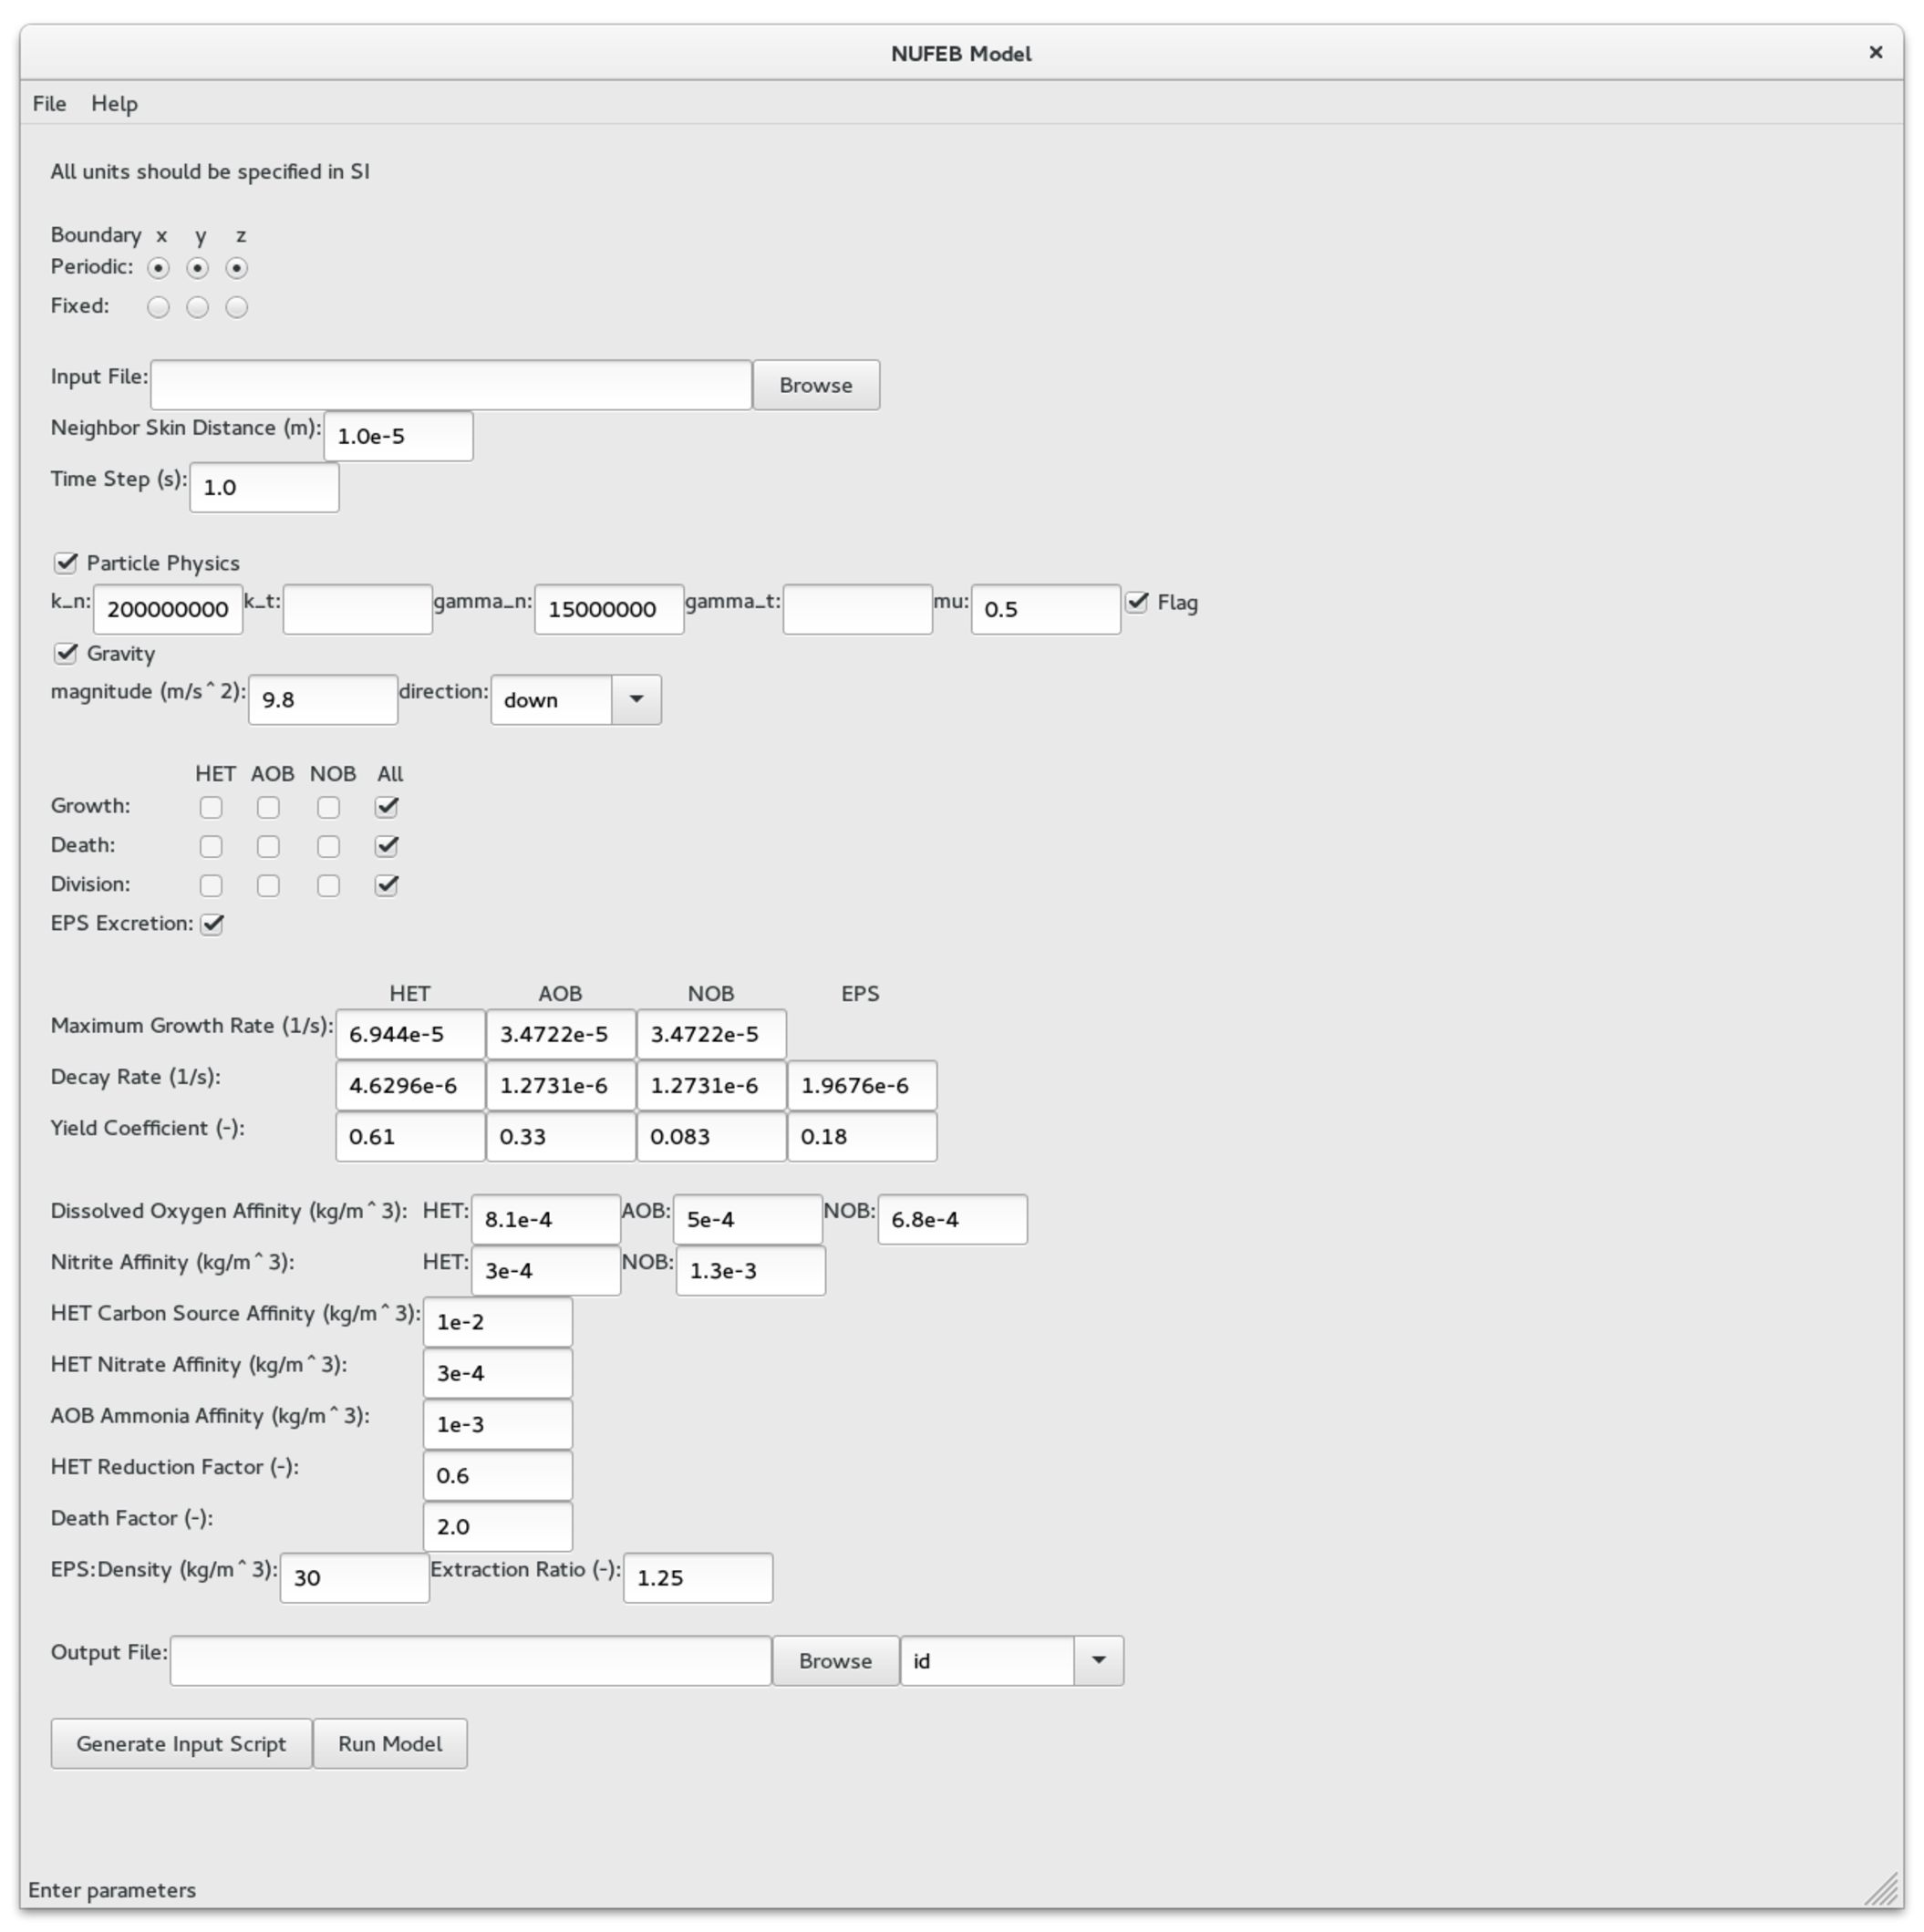
\includegraphics[width=0.9\columnwidth]{Figs/GUI.pdf}
\caption{Graphical User Interface (GUI) for NUFEB model}
\label{fig:GUI}       % Give a unique label
\end{center}
\end{figure}

\end{document}
